% !TEX encoding = UTF-8 Unicode
\documentclass[a4paper]{article}

\usepackage{color}
\usepackage{url}
\usepackage[utf8]{inputenc} % make weird characters work
\usepackage{graphicx}

%grafik
\usepackage{pgfplots}

%kraj dodavanja za grafik

\usepackage[english,serbian]{babel}

\usepackage[unicode]{hyperref}
\hypersetup{colorlinks,citecolor=green,filecolor=green,linkcolor=blue,urlcolor=blue}

\usepackage{listings}

\newtheorem{primer}{Primer}[section]
\providecommand{\keywords}[1]
{
  \small	
  \textbf{\textit{Ključne reči---}} #1
}

\definecolor{mygreen}{rgb}{0,0.6,0}
\definecolor{mygray}{rgb}{0.7,0.7,0.7}
\definecolor{mymauve}{rgb}{0.58,0,0.82}

\lstset{ 
  backgroundcolor=\color{white},   % choose the background color; you must add \usepackage{color} or \usepackage{xcolor}; should come as last argument
  basicstyle=\scriptsize\ttfamily,        % the size of the fonts that are used for the code
  breakatwhitespace=false,         % sets if automatic breaks should only happen at whitespace
  breaklines=false,                 % sets automatic line breaking
  captionpos=b,                    % sets the caption-position to bottom
  commentstyle=\color{mygreen},    % comment style
  deletekeywords={...},            % if you want to delete keywords from the given language
  escapeinside={\%*}{*)},          % if you want to add LaTeX within your code
  extendedchars=true,              % lets you use non-ASCII characters; for 8-bits encodings only, does not work with UTF-8
%  firstnumber=1000,                % start line enumeration with line 1000
  frame=single,	                   % adds a frame around the code
  keepspaces=true,                 % keeps spaces in text, useful for keeping indentation of code (possibly needs columns=flexible)
  keywordstyle=\color{blue},       % keyword style
  language=Python,                 % the language of the code
  morekeywords={*,...},            % if you want to add more keywords to the set
%  numbers=left,                    % where to put the line-numbers; possible values are (none, left, right)
%  numbersep=0pt,                   % how far the line-numbers are from the code
%  numberstyle=\tiny\color{mygray}, % the style that is used for the line-numbers
  rulecolor=\color{black},         % if not set, the frame-color may be changed on line-breaks within not-black text (e.g. comments (green here))
  showspaces=false,                % show spaces everywhere adding particular underscores; it overrides 'showstringspaces'
  showstringspaces=false,          % underline spaces within strings only
  showtabs=false,                  % show tabs within strings adding particular underscores
%  stepnumber=2,                    % the step between two line-numbers. If it's 1, each line will be numbered
  stringstyle=\color{mymauve},     % string literal style
  tabsize=2,	                   % sets default tabsize to 2 spaces
  title=\lstname                   % show the filename of files included with \lstinputlisting; also try caption instead of title
}

\renewcommand{\lstlistingname}{Kod}% Listing -> Algorithm
\renewcommand{\lstlistlistingname}{List of \lstlistingname s}%

\begin{document}

\title{Programski jezik Lua\\ \small{Seminarski rad u okviru kursa\\Metodologija stručnog i naučnog rada\\ Matematički fakultet}}

\author{Jovana Pejkić, Jana Jovičić, Katarina Rudinac, Ivana Jordanov \\  jov4ana@gmail.com, jana.jovicic755@gmail.com \\
rudinackatarina@gmail.com, ivanajordanov47@gmail.com}

\date{5.~april 2019.}

\maketitle

\abstract{
Pri rešavanju komplikovanih problema susrećemo se sa poteškoćom pri odabiru programskog jezika. Potrebno je da on bude fleksibilan, ali se ne bismo odrekli jednostavnosti ili dragocenog memorijskog prostora. Jedno od rešenja je programski jezik Lua. Cilj rada je da se pokaže kako je nastao ovaj programski jezik, kako se danas koristi i koje karakteristike poseduje. U te svrhe rad obuhvata opis njegovih fundamentalnih mehanizama, samim tim i načina kojim se složeni koncepti različitih programskih paradigmi posredstvom jednostavne semantike i svega 8 tipova podataka postižu u njemu.
} \\
\keywords{Lua, skript programski jezik, tipovi podataka}
\tableofcontents

% u svrhu najispravnijeg ocenjivanja svih clanova tima  
% imitiran je tag \beginAutor{} koji oznacava ko je radio koji deo 
% zavrsno ujednacavanje i strukturu rada radila je Jordanov Ivana

\newpage

\section{Uvod}
\label{sec:uvod}

%% \beginAutor{Katarina Rudinac}
 Lua spada u dinamički tipizirane, gradivne (eng. embeddable\footnote{embeddable language - klasa jezika koji se često koriste da prošire ili utiču na ponašanje postojeće aplikacije}) skript jezike. Podržava proceduralno, objektno orjektisano, funkcionalno i programiranje vođeno podacima\cite{bookUnix}.
%% \endAutor{KatarinaRudinac}
Nastao je kao potreba za fleksibilnim programskim jezikom koji će omogućiti jednostavno korišćenje nesrodnih mehanizama različitih programskih paradigmi, u jednoj zemlji u razvoju, a danas ima široku primenu u različitim oblastima programiranja. Koji su to mehanizmi i kako je nastala Lua biće opisano u poglavlju \ref{sec:nastanak} , dok će o njenoj primeni danas biti reči u poglavlju \ref{sec:primena}. Načini na koji su podržane funckionalna i objektno orjentisana paradigma biće spomenuti u poglavlju \ref{sec:paradigme}. Kao rezultat širenja brojna su okruzenja za Luu i njima će biti posvećeno celo poglavlje \ref{sec:okruzenja}. Jednostavnost programskog jezika će biti vidljiva kroz kodove koji demonstriraju ideju na kojoj je zasnovano programiranje u Lui (poglavlje \ref{sec:programiranje}), a pre toga u poglavlju \ref{sec:instalacija} biće date instrukcije za instalaciju.

\section{Nastanak}
\label{sec:nastanak}

%% \beginAutor{Katarina Rudinac}
Programski jezik Lua nastao je 1993. na Katoličkom univerzitetu u Rio de Žaneiru u Brazilu, i u prevodu sa portugalskog znači mesec. U okviru Tecgraf-a, grupe za razvoj tehnologija u računarskoj grafici (eng. Computer Graphics Technology Group), pri pomenutom univerzitetu, trojica naučnika zvanih Roberto Jeruzalimski, Luiz Henrike de Figereido i Valdemar Keles, svaki specijalizovan za različitu naučnu oblast, razvili su jezik Lua, i od tada pa do danas rade na njegovom održavanju i proširivanju.

\subsection*{Istorijski kontekst}


Zbog tadašnjih brazilskih zakona, koji su striktno ograničavali uvoz softvera i hardvera, favorizujući domaće proizvode i znatno otežavajući uvoz iz inostranstva (koji je bio dozvoljen samo ukoliko ne postoji adekvatna zamena, koju su proizvele domaće kompanije, što je bilo jako teško i komplikovano dokazati) stvorila se potreba za programskim jezikom nastalim u Brazilu. Lua se smatra jedinim programskim jezikom nastalim u nekoj zemlji u razvoju koji je dostigao globalnu popularnost, i pored Ruby nastalog u Japanu, jedinim značajnim jezikom nastalim van Evrope i severne Amerike.

\subsection*{Prethodnici jezika Lua}


Prethodnici Lue, dva mala programska jezika zvana DEL (Data Entry Language) i SOL (Simple Object Language, čija skraćenica u prevodu označava sunce, što je bila direktna inspiracija za naziv Lua), nastali su 1992. za potrebe brazilskog naftnog giganta Petrobrasa. Svrha naručenog grafičkog interfejsa je bila da olakša, ubrza i učini otpornijim na greške unos ogromne količine numeričkih podataka koji je morao biti unesen u zastarelom formatu nasleđenom iz doba bušenih kartica. 
%Ovaj interfejs je učinio unos podataka interaktivnim, kliktanjem na delove dijagrama, a potom prevodio ovako unesene podatke u potrebni format i automatski generisao izlazni fajl u tom formatu. Pored toga, program je vršio proveru unetih podataka i izračunavao određeni deo podataka koji više nije bilo potrebe ručno unositi. 
DEL je nastao kako bi se olakšalo pisanje ovih grafičkih interfejsa. Na razvoju ovog jezika radio je Luiz Henrike de Figerido.
%kao deklarativni jezik koji je opisivao svojstva i ograničenja polja za unos podataka i entiteta kojima su ta polja pripadala. Entiteti u DEL-u se mogu uporediti sa strukturama u nekom drugom jeziku. 

Paralelno sa razvojem DEL-a, razvijao se i PGM, na kojem su radili Roberto Jeruzalimski i Valdemar Keles. PGM je služio za ispis litoloških podataka i bilo je moguće ručno konfigurisati način ispisa. SOL je nastao kako bi se konfigurisanje olakšalo. SOL je završen marta 1993, ali nikada nije isporučen.

\subsection*{Nastanak jezika Lua}

Ubrzo je nastala potreba za dodatnim mogućnostima u okviru DEL-a i SOL-a, tako da su vođe timova iza ova dva projekta sredinom 1993. zaključili da bi najbolje bilo da se ova dva mini jezika integrišu u jedan. Odlučeno je da će biti potreban pravi programski jezik, koji će da sadrži naredbe dodele, kontrole toka, podrutine… Zbog toga što ogroman deo potencijalnih korisnika nisu profesionalni programeri, sintaksa i semantika je trebalo da budu što jednostavnije, a postojala je i potreba za opisom podataka kao u SOL-u. Portabilnost je takođe označena kao jedan od prioriteta. DEL nije direktno uticao na Luu kao jezik, već samo idejno, u smislu umetanja delova skript jezika u ogromne projekte. Mnogi koncepti u Lui pozajmljeni su iz drugih programskih jezika, uključujući Modulu, CLU, C++, SNOBOL i Awk (prikaz hronologije nastanka ovih programskih jezika dat je na slici \ref{fig:godine}, slika razvojnog stbla na slici \ref{fig:stablo}). %Operator tačka zarez je odlučeno da bude opcion.

U julu 1993, Valdermar je dovršio prvu implementaciju Lue, koja je veoma brzo doživela ogroman uspeh. Prevedena je korišćenjem lex i yacc alata i bila je izuzetno jednostavna. Od tada je izašlo ukupno pet verzija sa brojnim podverzijama, koje su redom dodavale nove funkcionalnosti, a vremenski intervali između verzija su postajali sve duži. U uvodu je opisano u koje kategorije programskih jezika spada Lua, a na razvojnom stablu, jezik Lua se nalazi kao naslednik Perl-a i Pascal-a.
 
%% \endAutor{Katarina Rudinac}


\begin{figure}[h!]
\begin{center}
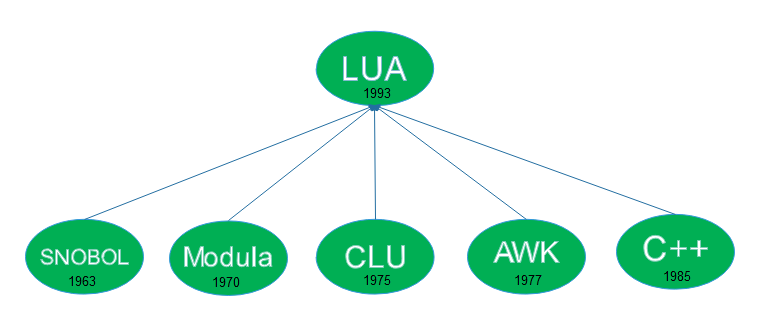
\includegraphics[scale=0.35]{godine.png}
\end{center}
\caption{Godine nastanka programskih jezika koji su uticali na Luu}
\label{fig:godine}
\end{figure}

\section{Primena}	
\label{sec:primena}

%% \beginAutor{Jana Jovicic}

Lua danas, zbog svoje jednostavnosti, efikasnosti i portabilnosti, ima primenu u najrazličitijim oblastima: ugradnim sistemima, mobilnim  uređajima, veb serverima i igricama. Koristi se na jedan od sledeća tri načina: kao skript jezik u sastavu aplikacija pisanih na nekom drugom jeziku, kao samostalan jezik ili zajedno sa C-om \cite{bookProgInLua}.

Ako se Lua upotrebljava u aplikaciji kao skript jezik, za njeno konfigurisanje potrebno je koristiti Lua-C API. Pomoću njega se mogu registrovati nove funkcije, praviti novi tipovi i vršiti izmene u ponašanju nekih operacija. Jedan od primera gde se Lua upotrebljava kao skript jezik je CGILua, alat za pravljenje dinamičkih veb stranica i manipulisanje podacima prikupljenih veb formama. U suštini, CGILua predstavlja apstrakciju za Veb server \cite{keplerProject}.

Kao skript jezik, Lua je našla primenu u razvoju softvera zasnovanom na komponentnom programiranju. U tom slučaju, Lua se koristi kao jezik za spajanje (eng. \textit{glue language}) postojećih komponenti višeg nivoa - komponenti koje su napisane u kompajliranom, statički tipiziranom jeziku (kao što je C ili C++). One obično predstavljaju koncepte niskog nivoa koji se neće mnogo menjati tokom razvoja programa jer oduzimaju mnogo procesorskog vremena. Osim spajanja takvih komponenti, Lua se koristi za pisanje onih delova koda koji će verovatno biti menjani mnogo puta i na taj način ubrzava proces razvoja programa \cite{bookProgInLua}.

Veliki broj programera se sve češće opredeljuje za Luu prilikom pravljenja igrica, pre svega zbog njene efikasnosti i lake integracije sa drugim programskim jezicima. O popularnosti Lue u domenu igrica govori činjenica da je 2003. godine, na osnovu rezultata anketa sprovedenih na GameDev.net sajtu, proglašena za jezik koji je najbolji za pisanje skriptova za igrice \cite{lua_news}. 

Još jedan primer u kome se Lua koristi zajedno sa drugim programskim jezicima je Adobe Photoshop Lightroom. Ona omogućava pisanje dodatnih softverskih komponenti koje mogu da se integrišu sa postojećim programom. Na primer, može da služi za pisanje komponenti kojima se kreiraju različiti efekati, za dodavanje stavki u menije i dijaloge, manipulaciju metapodacima i kreiranje novih tipova veb galerija \cite{adobe}.

Sve češće, Lua se koristi i kao samostalan jezik, čak i za veće projekte. U te svrhe su razvijene biblioteke koje nude različite funkcionalnosti. Na primer, postoje biblioteke za rad sa stringovima, tabelama, fajlovima, modulima, korutinama, matematičkim funkcijama itd. Sve one zajedno formiraju standardnu biblioteku Lue.

Treća mogućnost za upotrebu Lue je u okviru programa pisanih u C-u. Tada se ona importuje kao C biblioteka. U praksi, najveći deo programa je u C-u, a Lua se koristi za kreiranje interfejsa lakih za upotrebu.

%% \endAutor{Jana Jovicic}

\section{Podržane paradigme}
\label{sec:paradigme}

%% \beginAutor{Jana Jovicic}

Lua podržava različite paradigme, kao što su objektno-orjentisana, funkcionalna i proceduralna. Ona ne podržava ove paradigme pomoću specfičnih mehanizama za svaku od njih, već pomoću opštih mehanizama kao što su tabele, funkcije prvog reda, delegacija i korutine. Pošto ti mehanizmi nisu specifični ni za jednu određenu paradigmu, moguće su i druge paradigme. Svi mehanizmi Lue rade nad standardnom proceduralnom semantikom, što omogućuje njihovu laku integraciju. Prema tome, većina programa napisanih u Lui su proceduralni, s tim što uključuju i korisne tehnike drugih paradigmi \cite{multiParadigms} .

Podršku funkcionalnom programiranju u Lui pruža biblioteka Lua Fun, koja se još uvek razvija. Ona omogućava pisanje jednostavnog i efikasnog funkcionalnog koda korišćenjem funkcija višeg reda, poput map(), filter(), reduce(), zip(), itd. Primeri nekih funkcija iz ove biblioteke mogu se naći u dodacima \ref{dodaci}.

%% \endAutor{Jana Jovicic}

%% \beginAutor{Jovana Pejkic}

Iako Lua nije objektno-orjentisan jezik, on obezbeđuje sve objekte koji nam dopuštaju da implementiramo sistem objekata. Umesto klasa, u Lui pametna upotreba meta tabela može da kreira sistem klasa. Meta tabele mogu da kreiraju objekte zasnovane na prototipovima. Više o objektima u nastavku teksta.

%% endAutor{Jovana Pejkic}

\section{Okruženja}
\label{sec:okruzenja}

%% \beginAutor{Katarina Rudinac}

Tokom godina, nastala su brojna okruženja za jezik Lua, koja olakšavaju razvoj veb aplikacija. Korišćena su za razvoj mnogih poznatih sajtova i aplikacija, između ostalog i za Vikipedija sistem šablona, kao i kineski sajt za onlajn kupovinu Taobao.

Među najpopuilarnija Lua okruženja spadaju Lapis, Sailor, Luvit i Fengari.

Lapis je okruženje za pisanje veb aplikacija korišćenjem Lue ili Munskripta \footnote{eng. Moonscript --- programski jezik koji se kompajlira u Lui, a sa čitljivijom i kraćom sintaksom od njene} i izvršava se u okviru distribucije endžinIksa (eng. Nginx) zvane OpenResti (eng. OpenResty). OpenResti izvršava Lua (odnosno MunSkript) koristeći LuaJIT. Lapis je po svojoj funkcionalnosti analogan Reils (eng. Rails) okruženju za Rubi (eng. Ruby) i Laravel okruženju za PHP. Omogućava HTML templating, jednostavno uvođenje middleware-a, upravljanje ORM modelima (uključujući i migracije istih) i slično. 

Sailor okruženje je slično Lapisu ali razlikuje se po tome što uvodi dodatne, naprednije funkcionalnosti, od kojih je najvažnija mogućnost pisanja klijentskog koda u Lui, pomoću Lua virtuelne mašine implementirane u JavaScriptu. Još jedna prednost je što nije vezan za OpenResti, već ga je moguće izvršavati i na Apači, Endžiniksu, Mongus, Lajti, Savant i Luan (eng. Apache2, Nginx, Mongoose, Lighttpd, Xavante, Lwan redom) veb serverima. Naziv je inspirisan popularnom animiranom serijom zvanom ,,Sailor Moon'', naime kada je autorka okruženja, ucenica jednog od autora jezika, počela da uči Luu, rešila je da ako ikada napiše projekat u njoj, zvaće se Sailor, jer Lua znači mesec na portugalskom, kao što je gore pomenuto. Značajna je i po tome što je učenica jednog od autora Lue\cite{frameworkSailor}. 

Luvit je okruženje za Luu, koje implementira API identičan Node.js\cite{node_js} okruženju. Asinhrone I/O operacije se oslanjaju na istu biblioteku kao u Node.js-u (libuv). Zbog ove dve stvari, kod pisan za Luvit izgleda veoma slično kodu Node.js-a, stoga može biti pogodna polazna tačka za JavaScript/Node programere koji žele da nauče Luu. 

Fengari je implementacija Lua virtuelne mašine pisana u JavaScriptu. Izvršava se u veb pregledaču i omogućava izvršavanje Lua programa u tom okruženju. Lua kodu je dostupan kompletan API pregledača, uključujući i funkcije za manipulaciju DOM-a, pa može u potpunosti da zameni JavaScript pri pisanju klijentskog koda\cite{frameworkFengari}.

%% \endAutor{Katarina Rudinac}

\section{Instalacija}
\label{sec:instalacija}
  Lua je besplatna i pod MIT licencom \cite{licenca}.
Na Linuks (eng. Linux) i Mak (eng. Mac) operativnom sistemu, Lua bi trebalo da je već instalirana ili postoje paketi za nju. 

U slučaju instalacije, treba pratiti uputstva iz koda \ref{instalacija}. U zavisnosti od toga koja od platformi je najsrodnija onoj na kojoj se vrši instalacija, umesto ,,linux'' treba koristiti aix, bsd, c89, freebsd, generic, macosx, mingw, posix ili solaris. Interpreter se može koristiti i bez poslednjeg koraka \cite{lua_org}.

 Za Windows se preporucuje praćenje instrukcija sa zvanične stranice\footnote{zvanična strana: http://lua-users.org/wiki/BuildingLuaInWindowsForNewbies}. U svrhu izbegavanja instalacije Lue moguće je koristiti onlajn interpreter\footnote{link onlajn interpretera: http://lua-users.org/wiki/BuildingLuaInWindowsForNewbies}.

\begin{figure}

\begin{lstlisting}[caption={Instalacija iz terminala na linuxu},frame=single, label=instalacija]
# nacin 1:
sudo apt install lua5.3	                      #Debian/Ubuntu systems 
# yum install epel-release && yum install lua	#RHEL/CentOS systems 
# dnf install lua		                          #Fedora 22+

# nacin 2:
# instalacija potrebnih paketa ako ih vec nema:
sudo apt install build-essential libreadline-dev # Debian/Ubuntu
# yum groupinstall "Development Tools" readline	 # RHEL/CentOS systems 
# dnf groupinstall "Development Tools" readline	 # Fedora 22+

curl -R -O http://www.lua.org/ftp/lua-5.3.5.tar.gz #skida poslednju verziju
tar zxf lua-5.3.5.tar.gz # radi raspakivanje
cd lua-5.3.5             # pozicionira se u raspakovani folder 
make linux test          # kompajlira i testira
sudo make install        # instalira
\end{lstlisting}
\end{figure}

\section{Programiranje u Lui}
\label{sec:programiranje}

%% \beginAutor{Jana Jovicic}

Lua teži tome da bude fleksibilna, ali, takođe teži tome da bude mali jezik. Za ugradne jezike ovo je bitna osobina pošto se često koriste u uređajima koji imaju ograničene hardverske resurse. Kako bi se postigla ova dva suprotstavljena cilja, dodavanju novih karakteristika u jezik pristupa se ekonomično. Zbog toga Lua koristi malo mehanizama. A pošto ih je malo, oni moraju biti efikasni. Neki od takvih mehanizama su, na primer, tabele (opisane u poglavlju \ref{sec:tabele}), funkcije prvog reda (opisane u poglavlju \ref{sec:funkcije}), zatvorenja (opisana u poglavlju \ref{sec:zatvorenja}), iteratori (opisani u poglavlju \ref{sec:iteratori}) i refleksivne mogućnosti. Da bi jezik bio što manji, umesto hijerarhije numeričkih tipova (realni, racionalni, celi), Lua ima samo brojeve u pokretnom zarezu dvostruke preciznosti kao tip vrednosti \cite{multiParadigms}.
%% \endAutor{Jana Jovicic}
Lua ima ukupno 8 tipova: \textit{nil}, \textit{bool}, \textit{brojevi}, \textit{string}, \textit{korisnički podaci}, \textit{funkcije}, \textit{niti} i \textit{table}. U slučaju greške funkcija vraća nil i ono karakteriše odsustvo vrednosti. Nil nalazi primenu u brisanju promenljivih i oslobađanju memorije. Kada se promenljivoj dodeli nil, njena ranija vrednost biva izbrisana ukoliko ništa ne pokazuje na nju. Svaki tip može biti ,,kastovan'' u bool tako što se sve osim nil poima kao tačno. U tabeli \ref{kastovanje} su dati primeri nekih ishoda kastovanja u bool koji se razlikuju od, na primer, kastovanja u programskom jeziku C. U potpoglavljima biće više reči o nekim važnim konceptima ovog programskog jezika.

\begin{table}[h!]
\begin{center}
\begin{tabular}{|l|l|l|}
\hline
Tip & Vrednost & Bool vrednost \\
\hline
string &  ''čokolada'' &  true \\
\hline
string  & '''' &  true \\
\hline
number &  28 &  true \\
\hline
number & 0 &  true \\
\hline
nil &   & false \\
\hline 
\end{tabular}
\caption{Kastovanje u tip bool}
\label{kastovanje}
\end{center}
\end{table}

\subsection*{Tabele}
\label{sec:tabele}

%% \ beginAutor{Jovana Pejkic}

Tabele su dinamički kreirani asocijativni nizovi \footnote{Asocijativni niz je niz koji može biti indeksiran ne samo brojevima, već i stringovima ili bilo kojim drugim vrednostima, osim nil.}. Tabele se sastoje iz parova ključ-vrednost. Ako su ključevi tabele numerički, tabela predstavlja niz. Ako su ključevi ne-numeričke ili mešovite vrednosti, tabela je rečnik. Kao ključ u tabeli se može koristiti bilo šta, osim nil. Bilo šta, uključujuci i nil, može biti vrednost.
Program jedino preko referenci (ili pokazivača) njima manipuliše. Nema skrivenih kopija ili kreiranja novih tabela iza scene.

Tabela se kreira uz pomoć konstruktora. Nakon što je kreirana, tabelu treba dodeliti promenljivoj, u suprotnom na nju nije moguće referisati. Kada u programu ne postoji ni jedna referenca na neku tabelu, upravljač memorije će obrisati tu tabelu (i osloboditi memoriju koju je tabela zauzimala), tako da memorija koju je ta tabela zauzimala kasnije može biti ponovo upotrebljena. Tabela je relaciona struktura podataka koja skladišti vrednosti. Da bi se promenljiva sačuvala u tabeli, koristi se sledeća sintaksa:
\begin{verbatim}
table[key] = value
\end{verbatim}
Primer \ref{tabela1} demonstrira kako napraviti tabelu, sačuvati vrednost sa ključem x, i kako tu vrednost izvući iz tabele: %srediti kod
\begin{lstlisting}[caption={Primer čuvanja vrednosti u tabeli},frame=single, label=tabela1]
k = "x"
a[k]=10        --> nov ulaz, sa kljucem key="x" 
                           i vrednoscu value=10
a[20] = "great"--> nov ulaz, sa kljucem key=20 
                           i vrednoscu value="great"
print(a["x"])  --> ispisuje 10
k = 20
print(a[k])    --> ispisuje "great"
a["x"] = a["x"] + 1   --> uvecava ulaz "x"
print(a["x"])  --> ispisuje 11
\end{lstlisting}


\subsection*{Meta tabele i meta metodi}
Meta tabela je standardna tabela u Lui koja sadrži skup meta metoda koji mogu da promene ponašanje tabela. Meta metode su funkcije sa specifičnim imenom koje se pozivaju kada Lua izvršava određene operacije kao sto su sabiranje, konkatenacija stringova, poređenje itd. Na primer, koristeći meta tabele i meta metode, možemo definisati kako Lua računa izraz \textit{a + b}, gde su \textit{a} i \textit{b} tabele. Kad god Lua proba da sabere dve tabele, prvo proverava da li svaka od njih ima meta tabelu i da li ta meta tabela ima \textit{\_\_add} polje. Ako Lua pronadje to polje, poziva odgovarajuću funkciju za računanje sume.

Bilo koja tabela može biti meta-tabela bilo koje druge tabele. Grupa povezanih tabela može da deli zajedničku meta-tabelu (koja opisuje njihovo zajedničko ponašanje), a takođe tabela može biti svoja sopstvena meta-tabela (tako da opisuje svoje individualno ponašanje) \cite{bookProgInLua}.

\subsubsection*{Kreiranje meta tabele}
Za kreiranje meta-tabele neophodno je prvo kreirati običnu tabelu, a zatim njoj pridružiti odgovarajuće funkcije. U primeru \ref{meta2} obična tabela je nazvana \textit{meta}. Ovoj tabeli je pridružena funkcija koja se zove \textit{\_\_add}\footnote{\textit{\_\_add} je rezervisano ime za funkciju.}. \textit{\_\_add} funkcija prima dva argumenta: levi argument je tabela sa poljem koje se zove \textit{value}, a desni argument je broj:
\begin{lstlisting}[caption={Kreiranje meta-tabele i dodavanje meta-metoda \cite{bookProgInLua}},frame=single, label=meta2]
meta = { } 														-- kreira tabelu
meta.__add = function(left, right)		-- dodaje meta-metod
return left.value + right 						-- left je tabela
end
\end{lstlisting}
Zatim je napravljena nova tabela koja je nazvana \textit{container}. \textit{Container} tabela sadrži promenljivu nazvanu \textit{value}, koja ima vrednost \textit{5}:
\begin{lstlisting}[caption={Tabela \textit{container} \cite{bookProgInLua}},frame=single, label=meta3]
container = {
value = 5
}
\end{lstlisting}
Ako se u ovom trenutku pokuša sa dodavanjem broja 4 tabeli \textit{container}, Lua izbacuje sintaksnu grešku. Ovo se dešava zato što nije moguće tabeli dodati broj. Kod koji uzrokuje grešku prikazan je u primeru \ref{meta4}.
\begin{lstlisting}[caption={Neispravno sabiranje tabele i broja \cite{bookProgInLua}},frame=single, label=meta4]
result = container + 4 							-- neispravno
print ("result: " .. result)
\end{lstlisting}
Da bi ovaj kod bio ispravan potrebno je tabeli \textit{container} dodati meta-tabelu, koja ima \textit{\_\_add} meta-metod. Funkcija koja se koristi da tabeli dodeli meta-tabelu zove se \textit{setmetatable}. Ispravan kod dat je u primeru \ref{meta5}.
\begin{lstlisting}[caption={Ispravno sabiranje tabele i broja \cite{bookProgInLua}},frame=single, label=meta5]
setmetatable(container, meta) 			-- postavljanje meta-tabele
result = container + 4 							-- sada je ispravno
print ("result: " .. result)
\end{lstlisting}


%% \endAutor{Jovana Pejkic}


\subsection*{Funkcije}
\label{sec:funkcije}

%% \beginAutor{Jovana Pejkic}
Funkcije u Lui su vrednosti prve klase (eng. \textit{first-class values}) sa odgovarajućim ,,leksičkim opsegom''. Za funkciju se kaže da je vrednost prve klase ako ona ima ista prava kao i vrednosti poput brojeva i stringova. Funkcije mogu da se čuvaju u promenljivama (globalnim i lokalnim) i u poljima tabela, da se prosleđuju drugim funkcijama kao argumenti i da budu vraćene kao povratne vrednosti funkcija. Da funkcija ima ,,leksički opseg'' znači da može pristupati promenljivama funkcija kojima je okružena. Ova osobina omogućava da u Lui možemo da primenimo tehnike programiranja iz sveta funkcionalnih jezika kao i da program bude kraći i jednostavniji. Iako su funkcije vrednosti, postoji izraz kojim se funkcija kreira - deklaracija funkcije obično izgleda kao u primeru \ref{fun1}.
\begin{lstlisting}[caption={Deklaracija funkcije \cite{bookProgInLua}},frame=single, label=fun1]
    function foo (x) return 2*x end
\end{lstlisting}
Deklaracija funkcije započinje ključnom rečju \textit{function}, nakon koje sledi ime funkcije, a zatim lista parametara funkcije, koja može biti prazna ako funkciji nisu potrebni parametri. Nakon liste parametara piše se telo funkcije. Telo funkcije se završava navođenjem ključne reči \textit{end}.
Međutim, prethodni primer deklaracije funkcije samo je lepši način da se zapiše:
\begin{lstlisting}[caption={Dodela vrednosti tipa \textit{function} promenljivoj foo \cite{bookProgInLua}},frame=single, label=fun1]
    foo = function (x) return 2*x end
\end{lstlisting}
To jest, definicija funkcije je, u stvari, naredba koja promenljivoj dodeljuje vrednost tipa \textit{function}. Izraz sa desne strane operatora dodele se može posmatrati kao konstruktor za funkcije, baš kao što se vitičastim zagradama predstavlja konstruktor za tabelu. Rezultat takvog konstruktora funkcije zovemo anonimna funkcija. Iako se uglavnom funkcijama dodeljuju imena, postoje i situacije kada funkcije treba da ostanu anonimne. Na primer, biblioteka za tabele pruža funkciju \textit{table.sort}, koja prima tabelu i sortira njene elemente. Ova funkcija treba da omogući više varijacija sortiranja: rastuće ili opadajuće, numeričko ili alfabetsko, tabele sortirane po ključu, itd. Umesto kucanja posebnog koda da bi bile omogućene sve varijacije sortiranja, \textit{sort} pruza jedan (jedini) opcioni parametar, koji predstavlja funkciju za poređenje (engl. \textit{order function}), koja vrši poređenje dve vrednosti - prima dva elementa i vraća da li prvi argument treba da bude pre drugog. Primer \ref{fun2} prikazuje gde je zgodno upotrebiti anonimnu funkciju.
\begin{lstlisting}[caption={Primer tabele \cite{bookProgInLua}},frame=single, label=fun2]
     network = {
       {name = "grauna",  IP = "210.26.30.34"},
       {name = "arraial", IP = "210.26.30.23"},
       {name = "lua",     IP = "210.26.23.12"},
       {name = "derain",  IP = "210.26.23.20"},
     }
\end{lstlisting}
Da bi se vrednosti u tabeli sortirale po imenu polja u obrnutom alfabetskom poretku, kod treba da izgleda kao u primeru \ref{fun3}.
\begin{lstlisting}[caption={Sortiranje vrednosti tabele \cite{bookProgInLua}},frame=single, label=fun3]
    table.sort(network, function (a,b)
      return (a.name > b.name)
    end)
\end{lstlisting}
Funkciju, koja prima drugu funkciju kao argument, kao što je \textit{sort}, zovemo funkcijom višeg reda (eng. \textit{higher-order function}). Funkcije višeg reda predstavljaju mehanizam u programiranju, koji za kreiranje svojih argumenata često koristi anonimne funkcije. Funkcije višeg reda su posledica mogućnosti Lue da upravlja funkcijama kao vrednostima prve klase.

%% \endAutor{Jovana Pejkic}


\subsection*{Zatvorenja}
\label{sec:zatvorenja}

%% \beginAutor{Jovana Pejkic}

U Lui, promenljive koje su lokalne za neku funkciju su takođe dostupne u funkcijama koje su definisane unutar te funkcije, tj. unutar ugnježdenih definicija. Na primer, kada postoji neka funkcija koja vraća anonimnu funkciju, anonimna funkcija može da vidi lokalne promenljive funkcije kojom je okruzena. Međutim, nakon sto je anonimna funkcija vraćena, ona može da nadživi funkciju koja ju je vratila kreirajuci zatvorenje. Ovaj mehanizam dopušta pristup stanju funkcije omotača i nadpromenljivama\footnote{eng. upvalue - vrednost promenljive funkcije omotaca}, iako se funkcija omotac više ne izvršava.
Zatvorenje je funkcija, plus sve što joj je potrebno da pristupi njenim nadpromenljivama korektno. Ono što je vrednost u Lui je zatvorenje, a ne funkcija. Funkcija, sama za sebe, samo je prototip za zatvorenje.

%% \endAutor{Jovana Pejkic}

\subsection*{Iteratori}
\label{sec:iteratori}

%% \beginAutor{Jana Jovicic}

Iterator, konstrukcija koja omogćava prolazak kroz kolekciju, predstavlja se pomoću funkcije. Pri svakom pozivu, ta funkcija vraća naredni element iz kolekcije. U kodu \ref{iter1} dat je primer iteratora nad listom koji vraća vrednost elemenata liste.

\begin{lstlisting}[caption={Primer iteratora nad listom},frame=single, label=iter1]
function values (t)
	local i = 0
	return function () i = i + 1; return t[i] end
end

t = {10, 20, 30}
for element in values(t) do
	print(element)
end
\end{lstlisting}

Između uzastopnih poziva, iterator mora da pamti stanje u kom se nalazi kako bi znao da nastavi dalje odatle. U tu svrhu se koriste zatvorenja. \cite{lua_org_iterators}.

U kodu \ref{iter1} funckija omotač je values(). Pri svakom pozivu ona pravi zatvorenje (koje predstavlja sam iterator). To zatvorenje čuva svoje stanje u spoljašnjim promenljivama (\textit{t, i, n}) tako da, svaki put kada se pozove, vraća naredni element iz liste t. Kada više nema vrednosti u listi, vraća nil.

Postoje i iteratori bez stanja (eng. \textit{stateless iterators}). To su iteratori koji ne čuvaju sami svoja stanja, tako da možemo isti iterator iskoristiti u više petlji, bez potrebe da pravimo nova zatvorenja. U svakoj itreaciji, for petlja poziva svoj iterator sa dva argumenta: invarijantnim stanjem i kontrolnom promenljivom. Iterator bez stanja generiše naredni element na osnovu te dve vrednosti. U kodu \ref{iter2} prikazan je jedan iterator bez stanja - ipairs()\cite{bookProgInLua}.

\begin{lstlisting}[caption={Primer iteratora bez stanja},frame=single, label=iter2]
a = {"one", "two", "three"}
for i, v in ipairs(a) do
	print(i, v)
end
\end{lstlisting}
Rezultat izvrsavanja ovog programa je:
\begin{verbatim}
1	one
2	two
3	three
\end{verbatim}
Funkcija ipairs() vraća tri vrednosti: \textit{gen}, \textit{param}, i \textit{state} (koje se nazivaju iteratorski triplet). \textit{Gen} je funkcija koja generiše narednu vrednost u svakoj iteraciji. Ona vraća novo stanje (\textit{state}) i vrednost u tom stanju. \textit{Param} je trajni parametar \textit{gen} funkcije i koristi se za pravljenje instance \textit{gen} funkcije, npr. tabele. \textit{State} je privremeno stanje iteratora koje se menja nakon svake iteracije, npr. to je indeks niza\cite{luafun}. U kodu \ref{iter3} su prikazane ove tri vrednosti.
\begin{lstlisting}[caption={Primer iteratora bez stanja (nastavak)},frame=single, label=iter3]
a = {"one", "two", "three"}
gen, param, state = ipairs(a)
# rezultat izvrsavanja: function: 0x41b9e0	table: 0x1e8efb0	0
print(gen(param, state))
# rezultat izvrsavanja: 1	one
\end{lstlisting}


\subsection*{Primer jednostavnog koda}
\label{sec:primer_koda}

U ovom poglavlju će biti dat primer jednog jednostavnog koda u kom se može videti način na koje se koriste prethodno opisani elementi ovog programskog jezika. U primeru \ref{primer} je prikazano kako je moguće naći sve faktore broja koji se unosi sa standardnog ulaza. Od korisnika se prvo traži da unese broj, zatim se on učitava pomoću ugrađene funkcije \textit{io.read()} i poziva se korisnički definisana funkcija koja vraća tabelu svih faktora. U okviru te funkcije prvo je potrebno deklarisati praznu tabelu u koju će biti dodavani faktori. Zatim se u \textit{for} petlji proveravaju svi brojevi od 1 do korena prosleđenog broja, pri čemu je korak u iteriranju jednak 1. Ako taj broj deli prosleđeni broj, onda su on i broj koji se dobija deljenjem prosleđenog broja tim brojem faktori i dodaju se u tabelu pomoću funkcije \textit{insert()}. Zatim se tabela sortira i vraća kao rezultat funkcije. Na kraju, pri povratku iz funkcije, prolazi se kroz sve elemente tabele pomoću iteratora \textit{ipairs()} i oni se ispisuju na standardni izlaz. U ovom primeru se, takođe, može videti da se lokalne promenljive deklarišu ključom rečju \textit{local}. A prikazano je i pisanje jednolinijskih i višelinijskih komentara.

\begin{lstlisting}[caption={Primer izračunavanja faktora broja},frame=single, label=primer]
function get_all_factors(number)
    --[[--
    	Ova funkcija vraca sve faktore datog broja.
    	Preciznije, vraca tabelu koja sadrzi sve faktore.
    --]]--
    
    local factors = {}  -- Tabela u kojoj cuvamo faktore
    for possible_factor=1, math.sqrt(number), 1 do
        local remainder = number % possible_factor        
        if remainder == 0 then
           local factor1, factor2 = possible_factor,
           number/possible_factor
           table.insert(factors, factor1)
           table.insert(factors, factor2) 
        end
    end
    table.sort(factors)
    return factors
end

-- ovako se ispisuje poruka na standardni izlaz:
print("Unesite broj cije faktore zelite da izracunate:")
-- ovako se ucitava broj sa standardnog ulaza:
num = io.read("*n")
-- ovako se poziva funkcija:
factors_of_num = get_all_factors(num)
-- pomocu ipairs() iteratora se prolazi kroz kolekciju i ispisuje 
-- se svaki od faktora prosledjenog broja
for i, factor in ipairs(factors_of_num) do
   print(factor) 
end
\end{lstlisting}

%% endAutor{Jana Jovicic}

\section{Zaključak}
\label{sec:zakljucak}

U radu je pokazano kako Lua, iako je nastala za lokalne potrebe, danas ima primenu u svetu. Njena mala sintaksa navodi programere da raspolazući jednostavnim komponentama stvaraju efikasne algoritme, a jednostavnost sintakse se čuva iz verzije u verziju. Uprkos tome spektar načina njenog primenjivanja je širok. Lua se koristi u međusobno vrlo različitim projektima i na međusobno vrlo različite načine. Sve ove osobine svedoče tome da je Lua dobar izbor programskog jezika ne samo za spajanje raznorodnih projekata već i za započinjanje istih. Pored trenutnih mehanizama koje ima, u budućnosti bi ovaj jezik mogao dovesti do ideja za efikasniju implementaciju struktura podataka posredstvom tabela.

\addcontentsline{toc}{section}{Literatura}
\appendix
\bibliography{seminarski} 
\bibliographystyle{plain}

\appendix
\newpage
\section{Dodatak}
Opis funkcija koje su korišćene u primerima:
\label{dodaci}


\begin{enumerate}
  \item  fun.map(\textit{fun, gen, param, state})
  
  map() prihvata funkciju \textit{fun} i vraća novi iterator koji je nastao primenjivanjem funkcije \textit{fun} na svaki od elemenata tripletskog iteratora \textit{gen, param, state}. Mapiranje se vrši u prolazu kroz kolekciju, bez baferisanja vrednosti. Primer je dat u kodu \ref{map}. \cite{luafun}
   \begin{lstlisting}[caption={Primer funkcije map()},frame=single, label=map]
> each(print, map(function(x) return 2 * x end, range(4)))
2
4
6
8
\end{lstlisting}
  \item fun.filter(\textit{predicate, gen, param, state})
  
  filter() prihvata predikat \textit{predicate} na osnovu koga filtrira iterator predstavljen sa \textit{gen, param, state}. Vraća novi iterator za elemete koji zadovoljavaju predikat. Primer je dat u kodu \ref{filter}. \cite{luafun}
   \begin{lstlisting}[caption={Primer funkcije filter()},frame=single, label=filter]
> each(print, filter(function(x) return x % 3 == 0 end, range(10)))
3
6
9
\end{lstlisting}
\item fun.zip(iterator1, iterator2, ...)

   zip() prihvata listu iteratora i vraća novi iterator čija i-ta vrednost sadrži i-ti element iz svakog od prosleđenih iteratora. Povratni iterator je iste dužine kao najkraći prosledjeni iterator. Primer je dat u kodu \ref{zip}. \cite{luafun}
   \begin{lstlisting}[caption={Primer funkcije zip()},frame=single, label=zip]
> each(print, zip(range(5), {'a', 'b', 'c'}, rands()))
1       a       0.57514179487402
2       b       0.79693061238668
3       c       0.45174307459403
\end{lstlisting}
\end{enumerate}
\newpage
Slika razvojnog stabla:
\begin{figure}[h!]
\begin{center}
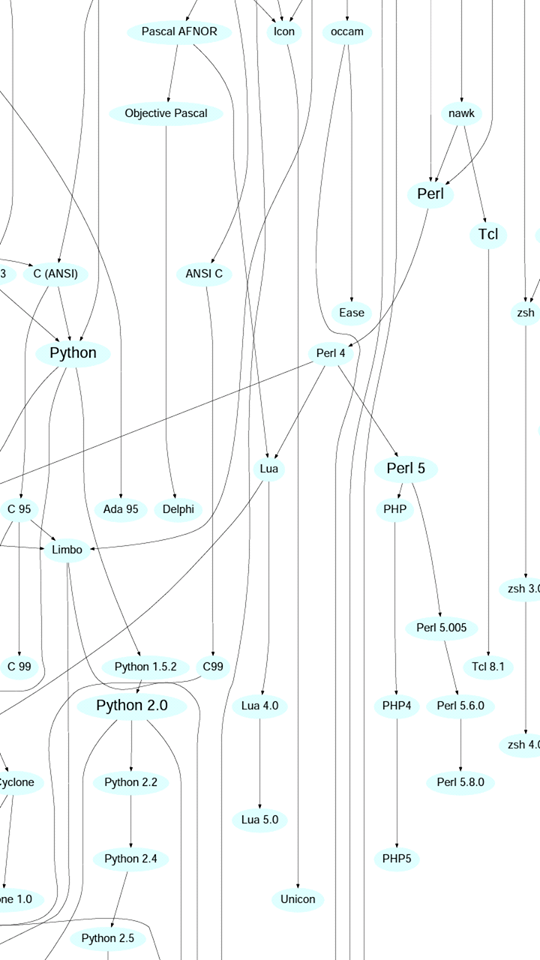
\includegraphics[scale=0.5]{stablo.png}
\end{center}
\caption{Razvojno stablo}
\label{fig:stablo}
\end{figure}


\end{document}
